% % % % % % % % % % % % % % % % % % % % % 
% numerical.tex - Ian Huston
% $Id: numerical.tex,v 1.51 2009/11/20 16:08:14 ith Exp $
% % % % % % % % % % % % % % % % % % % % % 
% Redefine CVSRevision for this section
\renewcommand{\CVSrevision}{\version$Id: numerical.tex,v 1.51 2009/11/20 16:08:14 ith Exp $}
% \input{numerical/paper3}

% % % % % % % % % % % % % % % % % % % % % % % % % % % % % % % % 
% =========================================================== %
% % % % % % % % % % % % % % % % % % % % % % % % % % % % % % % %
\chapter{Numerical System and Implementation}
\label{ch:numericalsystem}
% % % % % % % % % % % % % % % % % % % % % % % % % % % % % % % % 
% =========================================================== %
% % % % % % % % % % % % % % % % % % % % % % % % % % % % % % % %
% 
% 
% % % % % % % % % % % % % % % % % % % % % % % % % % % % % % % % 
% =========================================================== %
% % % % % % % % % % % % % % % % % % % % % % % % % % % % % % % %
\section{Introduction}
\label{sec:intro-num}
% % % % % % % % % % % % % % % % % % % % % % % % % % % % % % % % 
% =========================================================== %
% % % % % % % % % % % % % % % % % % % % % % % % % % % % % % % %

Our goal in Part~\ref{part:numerical} of this work is to show that, just as at first
order, a direct numerical calculation of the second order perturbations of a
scalar field system is achievable. 
In this chapter the implementation of this system is outlined.
The structure of the numerical
system follows the work done at first order by Martin
and Ringeval \cite{Martin:2006rs, Ringeval:2007am} and previously by
Salopek \etal \cite{Salopek:1988qh}.


The most important difference between an analytic and numerical treatment of the
equations presented in Chapter~\ref{ch:perts} is the requirement to specify a finite
numerical range of a finite number of $k$ modes to be calculated.
The upper cutoff in $k$, which marks the smallest scale considered, is well
motivated by the difficulty in observing primordial perturbations at very small
scales. 
On the other hand, we also need to specify the largest scale (or smallest $k$) that
we
will consider. Analytically, this is often taken to be the size of the universe,
with $k=0$ being the equivalent mode. One immediate problem with this
specification, however, is that
the Bunch-Davies vacuum initial conditions diverge. The standard approach to this
problem is to implement a cutoff
at large scales beyond which the amplitude of perturbations vanishes. This is a
pragmatic approach, but recently there has been some evidence that a sharp
cutoff similar to this could be responsible for the lack of power at large
scales in the WMAP data \cite{Lyth:2007jh, spergel, Sinha:2005mn,Kim:2009pf}.
 
The main concern is that the $k$ range covers most, if not all, of the modes observed
to date in the CMB. The WMAP team rely for their main results in 
\Rref{Komatsu:2008hk}  
 on $\ell$ multipoles in the range $\ell \in [3, 1000]$,
which corresponds approximately\footnotemark  to $k\in \left[0.92 \e{-60}, 3.1 \times
10^{-58}\right]\Mpl = \left[3.5\e{-4}, 0.12\right] \Mpc^{-1}$.
\footnotetext{The approximate conversion for $\ell$ is $\ell\simeq \frac{2k}{H_0}$ and a
Megaparsec
is given in Planck units as $1\Mpc^{-1} \simeq 2.6247\e{-57} \Mpl$.}
We will consider three different ranges of $k$ modes when producing the results in
Chapter~\ref{ch:results}, all of which contain the WMAP pivot scale
$\kwmap=0.002\Mpc^{-1}$. The
choice of $k$ range is flexible with the only numerical constraint being that the
number of modes at second order should be equal to $2^l +1$, where $l$ is a positive
integer. This enables
faster integration using the Romberg method, as explained below. 


In Chapter~\ref{ch:perts} the Klein-Gordon equations of motion were described for the
background field, and the first and second order field perturbations. These form the
basis of the numerical calculation in this chapter. In Section~\ref{sec:eqs-num},
these equations are rewritten in a form more amenable to numerical work. The time
variable is changed from conformal time, $\eta$, to the number of e-foldings, $\N$.
The convolution terms which are present in the Fourier space equations are then
written in terms of spherical polar coordinates and split into smaller units. 


Four inflationary potentials were chosen in order to test the numerical calculation.
These are defined in
Section~\ref{sec:pots-num} and the steps taken to establish the values of the
required parameters are outlined. The initial conditions used for the first order
perturbations are the Bunch-Davies vacuum conditions, as specified in
Section~\ref{sec:perts-intro}. At second order the perturbations are set to be
identically zero at the beginning of the simulation, as explained in
Section~\ref{sec:initconds-num}. This section also describes the method and timing of
the initialisation of the variables.


In Section~\ref{sec:impl-num} the numerical method is discussed. The calculation can
be split into four stages, each of which is described in depth along with the
logistical constraints and software environment. The numerical code is tested in
Section~\ref{sec:tests-num} by comparing the computed value with an analytic result
where this is possible. The choice of parameters in the calculation is determined by
the results of this comparison. In Section~\ref{sec:disc-numerical}, the results of
this chapter are summarised and discussed.


% % % % % % % % % % % % % % % % % % % % % % % % % % % % % % % % 
% =========================================================== %
% % % % % % % % % % % % % % % % % % % % % % % % % % % % % % % %
\section{Numerical Equations}
\label{sec:eqs-num}
% % % % % % % % % % % % % % % % % % % % % % % % % % % % % % % % 
% =========================================================== %
% % % % % % % % % % % % % % % % % % % % % % % % % % % % % % % %

The Klein-Gordon equations in Chapter~\ref{ch:perts} are not appropriate for a
numerical calculation and in this section we rearrange them into a more
suitable form. This involves a change of time coordinate and grouping of terms
into smaller units for calculation.
The second order slow roll equation \eqref{eq:KG2-fourier-sr-num} can be further
simplified by performing the $p$
integral and changing to spherical polar coordinates $q, \theta$ and $\omega$, where
$q=|\textbf{q}|$. The $\d^3q$ integral then becomes
% 
\begin{equation}
 \int \d^3q \longrightarrow \int_{0}^{\infty} q^2 \d q \int_{0}^{\pi}\sin \theta
\d\theta 
   \int_{0}^{2\pi}\d\omega \,.
\end{equation}
% 
For each $k$ mode equation we take the $\theta=0, \omega=0$ axis in the
direction of $\kvi$, so that the angle between $\kvi$ and $\qvi$ is
$\theta$, and the scalar product is $q_i k^i = q k \cos\theta$. 
The argument of
each $\dvp1$ or $\dvp1'$ term depends on $\theta$ through
$|\kvi-\qvi|=\sqrt{k^2 + q^2 -2kq \cos\theta}$ and
so must remain inside the $\theta$ integral. There is no $\omega$ dependence
in $\dvp1$ with this choice of axes, so the last integral is straightforward
to evaluate.

In the slow roll case there are only four different $\theta$ dependent terms,
here labelled $\A$--$\D$:
%
\begin{align}
\label{eq:AtoD-num}
 \A(\kvi,\qvi) &= \int_0^\pi \sin(\theta) \dvp1(\kvi-\qvi) \d\theta \,,
\nonumber\\
 \B(\kvi,\qvi) &= \int_0^\pi \cos(\theta)\sin(\theta) \dvp1(\kvi-\qvi)
\d\theta \,,\nonumber\\
 \C(\kvi,\qvi) &= \int_0^\pi \sin(\theta) \dvp1'(\kvi-\qvi) \d\theta \,,
\nonumber\\
 \D(\kvi,\qvi) &= \int_0^\pi \cos(\theta) \sin(\theta) \dvp1'(\kvi-\qvi)
\d\theta \,.
\end{align}
%
When written in terms of the variables defined in \eqs{eq:AtoD-num},
the slow roll equation
\eqref{eq:KG2-fourier-sr-num} becomes:
%
\begin{equation}
\label{eq:KG2-fourier-sr-aterms}
\dvp2''(\kvi)+2\H\dvp2'(\kvi)+k^2\dvp2(\kvi)
+\left(a^2
\Upp-{24 \pi G}(\vp_{0}')^2\right)
\dvp2(\kvi)
+ S(\kvi) = 0 \,,
\end{equation}
%
where $S(\kvi)$ is the source term which will be determined before the
second order system is run:
\begin{align}
\label{eq:KG2-src-sr-aterms}
&S(\kvi) = \frac{1}{(2\pi)^2}\int \d q\ \Bigg\{
a^2\Uppp q^2 \dvp1(\qvi) \A(\kvi,\qvi) \nonumber\\
&+ \frac{8\pi G}{\H}\vp_{0}' \Bigg[ 
\left( 3a^2\Upp + \frac{7}{2}q^4 + 2k^2q^2\right) \A(\kvi,\qvi)
-\left(\frac{9}{2} + \frac{q^2}{k^2}\right)kq^3 \B(\kvi,\qvi)
\Bigg]\dvp1(\qvi) \nonumber\\
%
&+ \frac{8\pi G}{\H}\vp_{0}' \Bigg[
-\frac{3}{2}q^2 \C(\kvi,\qvi) + \left(2-\frac{q^2}{k^2}\right)kq \D(\kvi,\qvi) 
\Bigg]\dvp1'(\qvi) \Bigg\} \,.
%
\end{align}
%
 The full set of equations which must be evolved are
then \eq{eq:KGback-num} for the background, \eq{eq:fokg} for the first
order perturbations and \eqs{eq:KG2-fourier-sr-aterms} and
\eqref{eq:KG2-src-sr-aterms} for the second order and source terms.


A more appropriate time variable for the numerical simulation is the
number of e-foldings \eqref{eq:nefolddefn-intro}. We employ 
%
\begin{equation}
\label{eq:def-ntime}
\N = \log ( a / a_{\mathrm{init}} )
\end{equation}
%
as our time variable instead of conformal time. This is measured from
$a_{\mathrm{init}}$, the value of $a$ at the beginning of the
simulation. We will use a dagger ($\dN{}$) to denote\footnotemark
differentiation with respect to $\N$ 
\footnotetext{This should not be confused
with the use of $^\dagger$ as Hermitian conjugate, which is confined to
Section~\ref{sec:perts-intro}.}.
% 
Derivatices with respect to conformal time, $\eta$, and coordinate time, $t$, are
then given by
%
\begin{align}
 \pd{ }{\eta} &= \frac{\d \N}{\d \eta}\pd{}{\N} = \H \pd{}{\N} \,,\\
 \pd{ }{t} &= \frac{\d \eta}{\d t} \frac{\d \N}{\d \eta}\pd{}{\N} = H
\pd{}{\N}\,,
\end{align}
%
respectively, where $H = \d \ln a/\d t$ and $\H = aH$.
% 

If $a$ is set to be unity at the present epoch, we can calculate
$a_{\mathrm{init}}$ once the background run is complete and the number of e-foldings
of inflation has been determined.
The value of $a$ at the end of inflation, $a_\mathrm{end}$, is calculated by
connecting it with $a_0$ (see for example
Eq.~(3.19) in \Rref{book:liddle} or Eq.~(7) in \Rref{Peiris:2008be}). 
This is given by
% 
\begin{equation}
 \label{eq:connection-num}
\frac{a_\mathrm{end}}{a_0} = \frac{a_\mathrm{end}}{a_\mathrm{reh}}
			     \frac{a_\mathrm{reh}}{a_\mathrm{eq}}
			     \frac{a_\mathrm{eq}}{a_\mathrm{0}}\,,
\end{equation}
% 
where $a_\mathrm{reh}$ and $a_\mathrm{eq}$ are the values of $a$ at the end of
reheating and matter-radiation equality. Using the relationship between energy
densities and the scale factor relevant to the matter and radiation dominated
eras, together with the Friedmann
equation \eqref{eq:Friedmann1-intro}, we can write
% 
\begin{equation}
 \label{eq:conn2-num}
\log\left(\frac{a_\mathrm{end}}{a_0}\right) =
 -\frac{2}{3}\log\left(\frac{H_\mathrm{end}}{\Mpl}\right)
 + \frac{1}{6}\log\left(\frac{H_\mathrm{reh}}{\Mpl}\right)
 + \frac{1}{2}\log\left(\frac{H_\mathrm{eq}}{\Mpl}\right)
 + \log\left(\frac{a_\mathrm{eq}}{a_0}\right)\,,
\end{equation}
% 
where $H_\mathrm{end}$, $H_\mathrm{reh}$ and $H_\mathrm{eq}$ are the values of $H$
at the end of inflation, at the end of reheating and at matter-radiation equality
respectively.
The value
of $a_\mathrm{eq}$ is taken to be $4.15\e{-5} (\Omega_m h^2)^{-1}$ and
$H_\mathrm{eq}=4.63\e{-54} \Omega_m^2 h^4 \Mpl$ \cite{Peiris:2008be, book:dodelson}.
The mean value for $\Omega_m h^2$ determined by WMAP5 + BAO + SN measurements is
$\Omega_m h^2 =0.1369$ \cite{Komatsu:2008hk}. With these values and taking
$a_0=1$, the scale factor at the end of inflation is given by
% 
\begin{equation}
\label{eq:aend-num}
a_\mathrm{end} \simeq e^{-72}
\left(\frac{H_\mathrm{end}}{\Mpl}\right)^{-\frac{2}{3}} 
\left(\frac{H_\mathrm{reh}}{\Mpl}\right)^{\frac{1}{6}}\,.
\end{equation}
% 


In Chapter~\ref{ch:results}, it is assumed that
reheating occurs instantaneously at the end of
inflation such that $H_\mathrm{reh} = H_\mathrm{end}$. This gives
$a_\mathrm{end} \simeq 10^{-29}$ and approximately 65
e-foldings from the end of inflation to the present. It also fixes the horizon
crossing
time of the WMAP pivot scale, $\kwmap=0.002\Mpc^{-1}$, to be about 60 e-foldings
before
the end of inflation. Because the Hubble parameter is not kept fixed during the
numerical calculation the
number of e-foldings between horizon crossing and the end of inflation will depend
on the form of the inflationary potential and the evolution of $H$. 


% 
The background and first order equations written in terms of the new time
variable $\N$ are
%
\begin{equation}
\ddN{\vp_{0}} + \left(3 + \frac{\dN{H}}{H}\right)\dN{\vp_{0}} + \frac{\Uphi}{H^2} = 0
\,,
\label{eq:bgntime}
\end{equation}
% 
and
% 
\begin{multline}
\ddN{\dvp1} + \left(3 + \frac{\dN{H}}{H}\right)\dN{\dvp1} 
 + \Bigg[ \left(\frac{k}{aH}\right)^2 + \frac{\Upp}{H^2} + \frac{8\pi G}{H^2}
 2\dN{\vp_{0}}\Uphi \\
% 
+ \left.\left(\frac{8\pi G}{H}\right)^2
\left(\dN{\vp_{0}}\right)^2\U \right]\dvp1 = 0\,, \label{eq:fontime}
\end{multline}
% 
respectively.
The corresponding second order perturbation equation takes the form
% 
\begin{multline}
 \label{eq:KG2-fourier-sr-ntime}
\ddN{\dvp2}(\kvi) + \left(3 + \frac{\dN{H}}{H}\right)
\dN{\dvp2}(\kvi)+ \left(\frac{k}{aH}\right)^2\dvp2(\kvi) \\
% 
+ \left(\frac{\Upp}{H^2}-{24 \pi G}(\dN{\vp_{0}})^2\right)
\dvp2(\kvi) +S(\kvi) = 0 \,,
\end{multline}
% 
with the source term given by
\begin{align}
\label{eq:KG2-source-ntime}
S(\kvi) = \frac{1}{(2\pi)^2}\int \d q\ &\Bigg\{
\frac{\Uppp}{H^2} q^2 \dvp1(\qvi) \A(\kvi,\qvi) \nonumber\\
&+\, \frac{8\pi G}{(aH)^2}\dN{\vp_{0}} \Bigg[ 
\left( 3a^2\Upp q^2 + \frac{7}{2}q^4 + 2k^2q^2\right) \A(\kvi,\qvi) \nonumber\\
% 
&-\left(\frac{9}{2} + \frac{q^2}{k^2}\right)kq^3 \B(\kvi,\qvi)
\Bigg]\dvp1(\qvi) \nonumber\\
%
&+\, 8\pi G \dN{\vp_{0}} \Bigg[
-\frac{3}{2}q^2 \tilde{\C}(\kvi,\qvi) + \left(2-\frac{q^2}{k^2}\right)kq
\tilde{\D}(\kvi,\qvi) 
\Bigg]\dN{\dvp1}(\qvi) \Bigg\}\,,
%
\end{align}
%
where 
%
\begin{align}
\label{eq:cdtilde-num}
 \tilde{\C}(\kvi,\qvi) &= \frac{1}{aH} \C(\kvi-\qvi) = \int_0^\pi \sin(\theta)
\dN{\dvp1}(\kvi-\qvi) \d\theta \,,\nonumber \\
 \tilde{\D}(\kvi,\qvi) &= \frac{1}{aH} \D(\kvi-\qvi) = \int_0^\pi \cos(\theta)
\sin(\theta) \dN{\dvp1}(\kvi-\qvi)
\d\theta \,.
\end{align}



The arguments of $\dvp1$ and $\dN{\dvp1}$ in the $\A$--$\tilde{\D}$ terms require
special consideration. 
To compute the integrals, $\theta$ is sampled at 
% 
\begin{equation}
\label{eq:nthetadefn}
N_\theta = 2^l + 1
\end{equation}
% 
points in the range
$[0,\pi]$ (for some $l\in \mathbb{Z}^+$ to allow Romberg integration) and the
magnitude of
$\kvi-\qvi$
is
found using
% 
\begin{equation}
 |\kvi -\qvi| = \sqrt{k^2 + q^2 - 2kq\cos(\theta)}\,.
\end{equation}
%
While $\dvp1(\kvi)=\dvp1(k)$, the value of $|\kvi-\qvi|$ is at most
$2\kmax$, where $k,q \in [\kmin,\kmax]$. This means that to calculate
the source term for the $k$ range described we require that $\dvp1$
and $\dN{\dvp1}$ be known in the range $[0, 2\kmax]$. In
Section \ref{sec:impl-num}, we will 
show that this first order upper bound does not significantly affect
performance. On the other hand, $|\kvi-\qvi|$ can also drop below the
lower cutoff of calculated $k$ modes. As discussed above a sharp cutoff will be
implemented and $\dvp1(k)=0$ used for the values below
$\kmin$. When the spacing of the discrete $k$ values, $\Delta k$,  is
approximately $\kmin$ the cutoff affects only the $k=q$ modes and
is only significant close to $\kmin$. 
Section \ref{sec:tests-num}
describes how the accuracy is affected by changing $\Delta k$ and
other parameters. Without extrapolating outside our computed $k$ range
it appears to be very difficult to avoid taking $\dvp1=0$ for a small number of
$k$ values below $\kmin$.


The value of $|\kvi-\qvi|$ will not in general coincide with the computed $k$
values of $\dvp1$. We use linear interpolation between the neighbouring $k$'s to
estimate the value of $\dvp1$ at these points. We leave to future work the
implementation of a more
accurate and numerically more intensive interpolation scheme.


Throughout the discussion above we have not specified any particular inflationary
potential, $V$. Indeed the numerical code can use any reasonable
single field potential provided that it drives a period of inflationary expansion in
the e-folding range being simulated. In the next section the four potentials which
have been tested are outlined. 

% % % % % % % % % % % % % % % % % % % % % % % % % % % % % % % % 
% =========================================================== %
% % % % % % % % % % % % % % % % % % % % % % % % % % % % % % % %
\subsection{Potentials and Parameters}
\label{sec:pots-num}
% % % % % % % % % % % % % % % % % % % % % % % % % % % % % % % % 
% =========================================================== %
% % % % % % % % % % % % % % % % % % % % % % % % % % % % % % % %
\begin{table}[htb]
\begin{center}
\begin{tabular}{ccc}
\toprule
Potential & Parameter & Value\\
\midrule
$\msqphisq$ & $m$ & $6.32\e{-6}\Mpl$\\
$\lambdaphifour$ & $\lambda$ & $1.55\e{-13}$\\
$\phitwooverthree$ & $\sigma$ & $3.82\e{-10}\Mpl^{\frac{10}{3}}$\\
$\msqphisqwithV$ & $m_0$ & $1.74\e{-6}\Mpl$\\
\bottomrule
\end{tabular}
\caption[Parameter values]{The parameter values for the four potentials, chosen so
that $\Pr(\kwmap)$ is in agreement with the WMAP5 value.}
\label{tab:params-num}
\end{center}
% 
\end{table}

To demonstrate the numerical calculation four different single field slow roll
potentials were chosen. These are not intended to represent an exhaustive selection,
but they do exhibit an interesting variety of behaviours. The potentials used are:
% 
% 
\begin{enumerate}
% 
 \item $V(\vp) = \msqphisq$. This is the original chaotic inflation model which is
still in good agreement with the observational data \cite{Alabidi:2008ej}.
% 
 \item $V(\vp) = \lambdaphifour$. Although increasingly in tension with observations
 this is a standard large field model.
% 
 \item $V(\vp) = \phitwooverthree$. This potential with an unusual fractional index
is the effective potential resulting from the monodromy inflation model of D$4$
branes, where observable tensor modes are possible \cite{Silverstein:2008sg,
Alabidi:2008ej}.
% 
 \item $V(\vp) = \msqphisqwithV$. This hybrid inflation model requires inflation to
be terminated by the decay of another field. However, this will not be
implemented in the code. Instead,
inflation will be set by hand to end when $\vp \simeq 8$. By taking a value of
$U_0 = 5\e{-10}\Mpl^{4}$ a blue spectrum ($n_s>1$) can then be obtained
\cite{Linde:1993cn,Komatsu:2008hk}.
% 
\end{enumerate}
% 
% 
\begin{figure}[htbp]
\centering%
\subfloat[$V(\vp)=\msqphisq$]{
 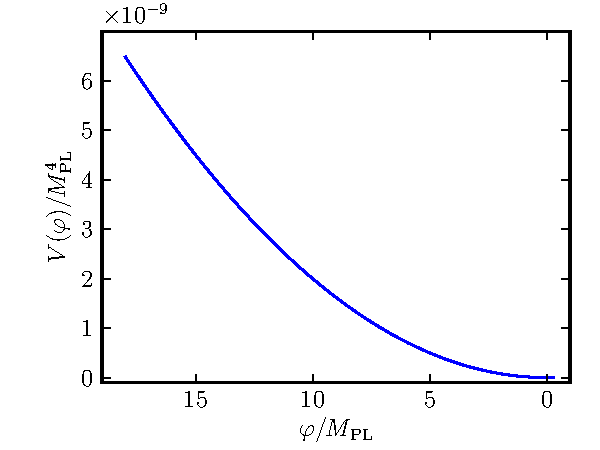
\includegraphics[width=0.43\textwidth]{numerical/graphs/msqphisq_potential-small}
}\qquad%
\subfloat[$V(\vp)=\lambdaphifour$]{
 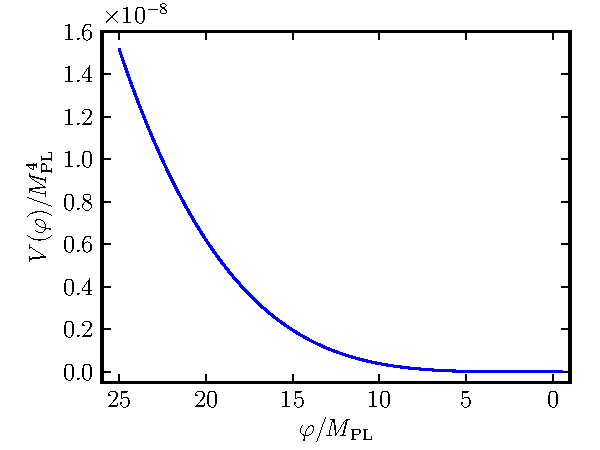
\includegraphics[width=0.43\textwidth]{numerical/graphs/lambdaphi4_potential-small}
}\\%
\subfloat[$V(\vp)=\phitwooverthree$]{
 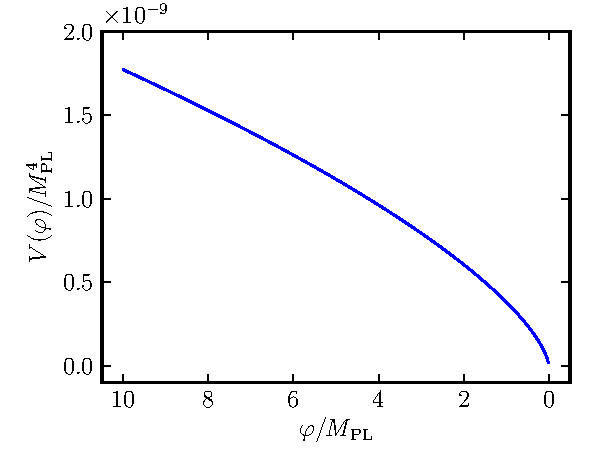
\includegraphics[width=0.43\textwidth]{numerical/graphs/phi2over3_potential-small}
}\qquad%
\subfloat[$V(\vp)=\msqphisqwithV$]{
 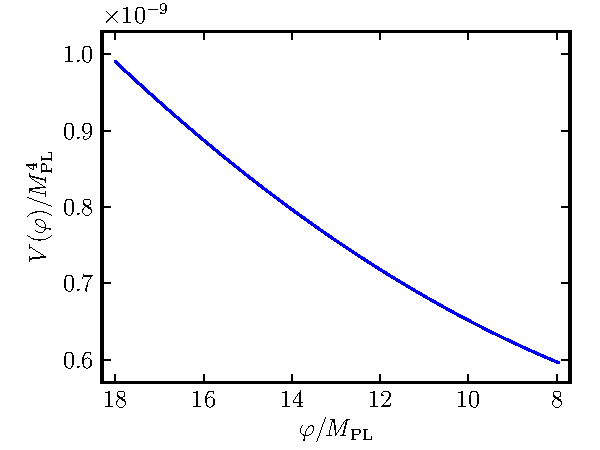
\includegraphics[width=0.43\textwidth]
  {numerical/graphs/msqphisq_withV0_potential-small}
}
\caption[Different potentials used]{Plots of the four different potentials used.}
\label{fig:potentials-num}
\end{figure}
% 
% 
In Figures~\ref{fig:potentials-num} and \ref{fig:cmp-pot-num} the potentials are
plotted over the course of their evolution. Throughout the rest of this
chapter we will use $V(\vp)=\msqphisq$ to
demonstrate the calculation unless otherwise stated. In Chapter~\ref{ch:results} the
results for each potential will be compared.



\begin{figure}[htbp]
\centering%
\subfloat[The potentials in terms of $\varphi$.][The potentials in terms of
$\varphi$ over the course of the background evolution.]{
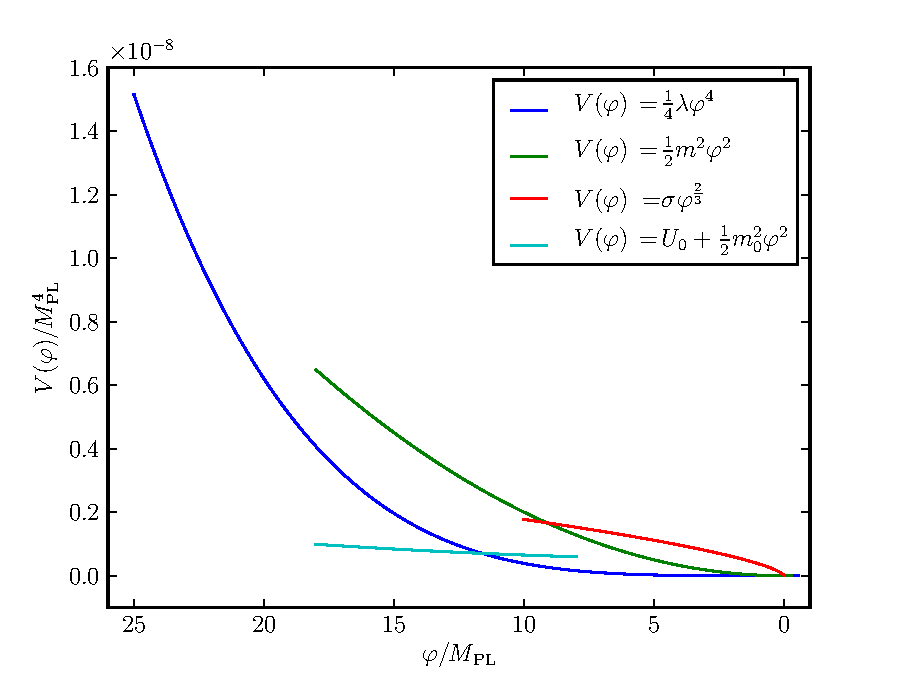
\includegraphics[width=0.8\textwidth]
  {numerical/graphs/cmp_pot_phi-large}
}\\%
\subfloat[The potentials in terms of $\N$.][The potentials in terms of $\N$ for the
last 70 e-foldings of inflation.]{
 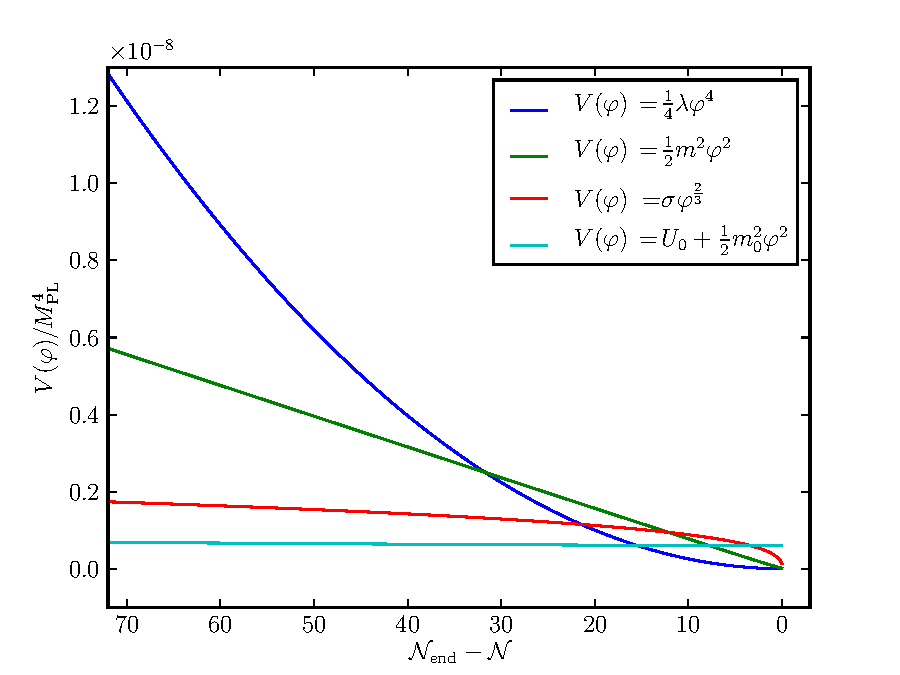
\includegraphics[width=0.8\textwidth]
  {numerical/graphs/cmp_pot_n-large}
}
\caption[Comparison of potentials]{A comparison of the four different potentials
used.}
\label{fig:cmp-pot-num}
\end{figure}


For each of the chosen potentials there is one free parameter that needs to be
determined.
We choose the parameters $m$, $\lambda$, $\sigma$ and $m_0$ so that $\Pr$ calculated
for each model is in agreement with the
WMAP5 value at the pivot scale
$\kwmap=0.002\Mpc^{-1} \simeq5.25\times10^{- 60} \Mpl$. 
The dependence of $\Pr(\kwmap)$ on each of the parameters can be seen in
Figure~\ref{fig:params-num}.
Requiring $\Pr(\kwmap)=2.457\e{-9}$
gives the values shown in Table~\ref{tab:params-num}. Here we have chosen the lower
of the two possible values of $m_0$ shown in Figure~\ref{fig:mv0-params-num}.



\begin{figure}[htbp]
\centering%
\subfloat[Fixing $m$ for $V(\vp)=\msqphisq$.]{
 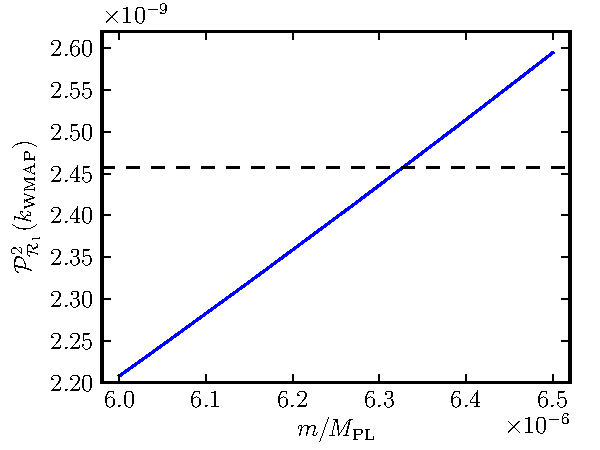
\includegraphics[width=0.43\textwidth]{numerical/graphs/msqphisq_params-small}
}\qquad%
\subfloat[Fixing $\lambda$ for $V(\vp)=\lambdaphifour$.]{
 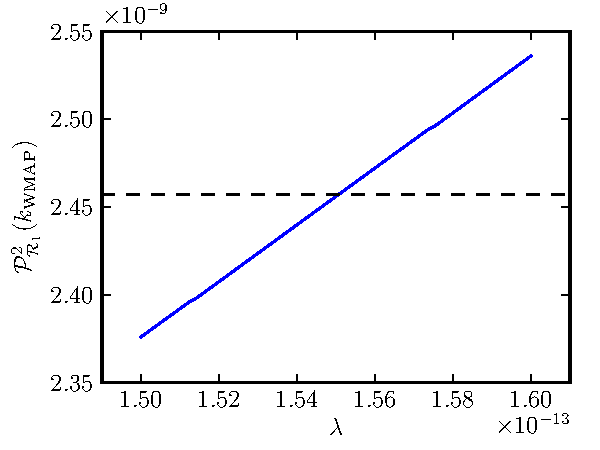
\includegraphics[width=0.43\textwidth]{numerical/graphs/lambdaphi4_params-small}
}\\%
\subfloat[Fixing $\sigma$ for $V(\vp)=\phitwooverthree$.]{
 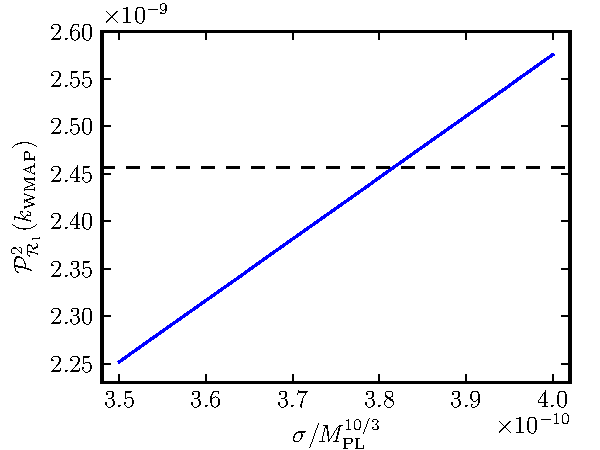
\includegraphics[width=0.43\textwidth]{numerical/graphs/phi2over3_params-small}
}\qquad%
\subfloat[Fixing $m$ for $V(\vp)=\msqphisqwithV$.]{
 \label{fig:mv0-params-num}
 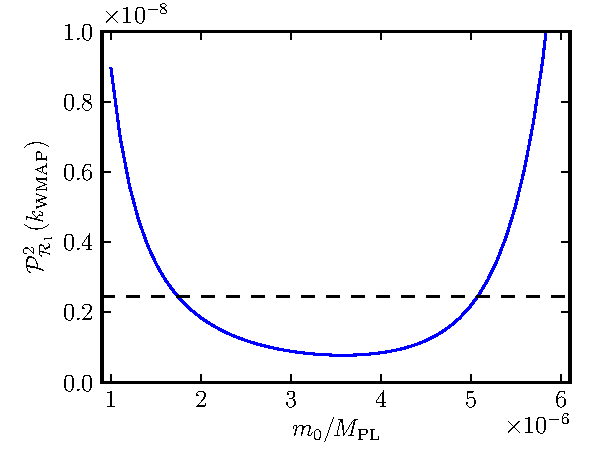
\includegraphics[width=0.43\textwidth]
  {numerical/graphs/msqphisq_withV0_params-small}
}
\caption[Parameter values for different potentials]{Parameter values for the
different potentials are chosen by requiring consistency with the WMAP5
normalisation of the power spectrum.}
\label{fig:params-num}
\end{figure}


% % % % % % % % % % % % % % % % % % % % % % % % % % % % % % % % 
% =========================================================== %
% % % % % % % % % % % % % % % % % % % % % % % % % % % % % % % %
\subsection{Initial Conditions} 
\label{sec:initconds-num}
% % % % % % % % % % % % % % % % % % % % % % % % % % % % % % % % 
% =========================================================== %
% % % % % % % % % % % % % % % % % % % % % % % % % % % % % % % %

The background system requires initial conditions for $\vp_{0}$ and
$\dN{\vp_{0}}$. These initial conditions and the range of
e-foldings to be simulated must be selected with the choice of
potential in mind. Not only must the
e-folding range include an inflationary period, but the $k$ modes to
be calculated at first and second order must begin inside the horizon. For example,
the initial value $\vp_0 = 18\Mpl$ for the
$\msqphisq$ model 
gives the background evolution described below and shown in Figure~\ref{fig:eps}. As
the evolution quickly reaches the attractor solution, the choice for $\dN{\vp_0}$
is not particularly important; changing the initial value adds or subtracts a small
number of e-foldings of evolution before the modes are initialised
\cite{Ringeval:2007am, Martin:2006rs}.


The initial conditions are set for each $k$ mode a few e-foldings
before horizon crossing. This follows Salopek
\etal
\cite{Salopek:1988qh} and is justified on the basis that the mode is
sufficiently far inside the
horizon for the Minkowski limit to be taken. This initial time,
$\N_{\mathrm{init}}(k)$, is calculated to be when
%  
\begin{equation}
 \frac{k}{(aH)|_{\mathrm{init}}} = 50 \,.
\end{equation}
%
The range of e-foldings being used must include the starting point for
all $k$ modes, but the parameter on the right hand side, here chosen to
be 50, can be changed if needed.  We use the small wavelength solution
of the first order equations described in Section~\ref{sec:perts-intro} as the
initial conditions \cite{Salopek:1988qh}, with
%
\begin{align}
\label{eq:foics}
 \dvp1|_{\mathrm{init}} &= \frac{\sqrt{8\pi G}}{a}
\frac{e^{-i k\eta}}{\sqrt{2k}} \,,\\
 \dN{\dvp1}|_{\mathrm{init}} &= -\frac{\sqrt{8\pi G}}{a}
\frac{e^{-i k\eta}}{\sqrt{2k}} \left(1 + i \frac{k}{a H}\right) \,,
\end{align}
%
where conformal time $\eta$ can be calculated from 
% 
\begin{equation}
\label{eq:etacalc-num}
\eta=\int \d\N/aH \simeq
-(aH(1-\bar{\varepsilon}^2_H))^{-1}\,,
\end{equation} 
% 
when $\bar{\varepsilon}_H$ changes slowly. For
example $\kwmap$ is initialised
about $65$ e-foldings before the end of inflation and crosses the horizon about $5$ e-foldings
later.
We also use these formulae in the calculation of the source term in \eq{eq:KG2-source-ntime} to
determine the value of $\dvp1$ for a $k$ mode before its numerical evolution has
begun.


We are interested in the production of second order effects by the
evolution of the the Gaussian first order modes and we make no
assumptions about the existence of second order perturbations before
the simulation begins. Therefore, we set the initial condition for each second order
perturbation mode to be $\dvp2=0, \dN{\dvp2}=0$ at
the time when the corresponding first order perturbation is initialised.



% % % % % % % % % % % % % % % % % % % % % % % % % % % % % % % % 
% =========================================================== %
% % % % % % % % % % % % % % % % % % % % % % % % % % % % % % % %
\section{Implementation} 
\label{sec:impl-num}
% % % % % % % % % % % % % % % % % % % % % % % % % % % % % % % % 
% =========================================================== %
% % % % % % % % % % % % % % % % % % % % % % % % % % % % % % % %


The current implementation of the code is mainly in the Python\footnote{Python
website: \url{http://www.python.org}} programming language (with compiled Cython
components) and uses the
Numerical and Scientific Python modules for their strong compiled array support
\cite{scipy}. The core of the model computation is a
Runge-Kutta fourth order method (see, for example, Eq.~(25.5.10) in
\cite{abramowitz+stegun}).  Following
Refs.~\cite{Martin:2006rs} and \cite{Ringeval:2007am} the numerical calculation
proceeds in four stages. The background equation (\ref{eq:bgntime}),
rewritten as two first order equations, is
evolved from the specified initial state until some end time required
to be after the end of the inflationary regime.  The end of inflation
occurs when $\d^2a/\d t^2$ is no longer positive and the parameter
$\bar{\varepsilon}^2_H = \varepsilon_H= -\dN{H}/H$ becomes greater than or
equal to unity
(see Figure~\ref{fig:eps}). This specifies a new end time for the first
order run, although the simulation can run beyond the strict end of
inflation if required. For the $V(\vp)=\msqphisqwithV$ model, the end of inflation is
set by hand to remove the need for a second, inflation-terminating field. The initial
conditions for the first order system are then set as above.
%
\begin{figure}[htbp]
\centering
 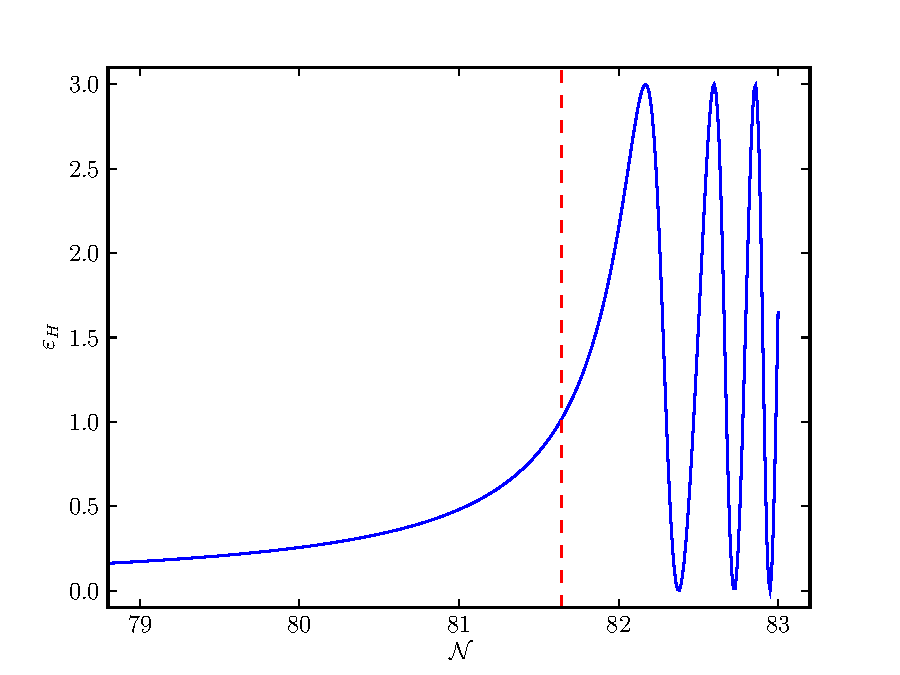
\includegraphics[width=0.8\textwidth]{./numerical/graphs/bgepsilon}
 \caption[Plot of $\varepsilon_H$ near the end of inflation]{The end of
inflation is
determined by calculating when
   $\bar{\varepsilon}^2_H = \varepsilon_H=-\dN{H}/H=1$ (red dashed line). Along the
$x$-axis,
   $\N$ is the number of e-foldings from the start of the
   simulation.}
\label{fig:eps}
\end{figure}


The system of ordinary differential equations for the first order
perturbations in \eq{eq:fontime} is integrated using a standard fourth order
Runge-Kutta method. A fixed time step method is used in order to
simplify the construction of the  second order source term.
This is also necessary since it is not known a priori
which time steps would be required at
second order if an adaptive time step system were used. The first
order equations are separable in terms of $k$ and so it is
straightforward to run the system in parallel and collate
the results at the end. However, as will be discussed below, the first
order calculation is not computationally expensive in comparison with
the other stages and only takes of the order of a few minutes for around
$8000$ time steps with $\Delta \N=0.01$ and $1025$ $k$ modes.


Once the first order system has been solved, 
the source term for the second order system must be calculated. As the
real space equation for the source involves terms quadratic in the
first order perturbation, it is necessary to perform a convolution in
Fourier space, as shown in \eq{eq:KG2-fourier-sr-aterms}.  We do not transform
back into real space due to the presence of both
gradient operators and their inverses. 
Instead, the slow roll version of
the source term integrand was used, although it is worth remarking that the method
can also be
applied to the full equation. This stage is computationally the most
intensive, and can be run in parallel since the calculation at each time step is
independent of the others. The nature of the convolution integral and the
dependence of the first order perturbation on the absolute value of
its arguments requires that twice as many $k$ modes are calculated at
first order than are desired at second order.  As
the first order calculation is computationally cheaper than the source
term integration, this does not significantly lower the possible
resolution in $k$-space, which is still limited by the source term
computation time.  Once the integrand is determined, it is fed into a
Romberg integration scheme. As for $\theta$,  which was
discretised by $N_\theta$ points in \eq{eq:AtoD-num}, this requires that the
number of $k$ modes is
%
\begin{equation}
\label{eq:nk-constraint-num}
N_k=2^l + 1\,,
\end{equation}
%
for some\footnotemark $\,l\in\mathbb{Z}^+$. 
\footnotetext{The number of discretised $k$ modes $N_k$ does not need to be equal to
  $N_\theta$.}
This requirement can be relaxed by opting for a less
accurate and somewhat slower standard quadrature routine.


The second order system is finally run with the source term and other
necessary data being read as required from the memory or disk. The
Runge-Kutta method calculates half time steps for each required point.
For example, if $y(x_n)$ is known and $y(x_{n+1})=y(x_n+h)$ is required
(for step size $h$), the method will calculate the derivatives of $y$
at $y(x_n), y(x_n +h/2)$ and $y(x_n + h)$. As we need to specify the
source term at every calculated timestep, the requested timestep for
the second order method must be twice that used at first order.  This decreases the
accuracy of the method but does not require the use
of splines and interpolation techniques to determine background and
first order variables between time steps.


The second order system is similar in run time to the first order 
system. However, the
source integration is more complex and involves the
integration of $N_k^2\times N_\theta$ values at
each time step.
When $N_k=1025$ and $N_\theta=513$, the first order evolution lasts around 200
seconds. The source calculation, on the other hand, takes approximately 200 seconds
for each time step. Each of the four terms $\A-\wt{\D}$ is approximately 16 gigabytes
in size at each time step for these values of $N_k$ and $N_\theta$. However, only the
integrated result is stored for use
in the second order run. This is approximately $16$ kilobytes in size for each time
step. 
Results for each stage are stored in the open HDF5 standard
\cite{pytables, hdf5}, which can
deal efficiently with large
files, is very portable and allows for data analysis independent of the
Python/Numpy programming environment.

The full calculation contains around 8000 timesteps, making the source term
calculation approximately 470 hours long. Each time step in independent of the
others, however, so parallelisation of the system is straightforward. The results in
Chapter~\ref{ch:results} were obtained on the Virgo Cluster in the Astronomy Unit at
Queen Mary, University of London. The code was run on ten nodes, each containing
four Opteron cores with a clock speed of $1994$Mhz. With this configuration the run
time of the source term calculation is reduced to under twelve hours. 



% We intend to release the program under a suitable license once the code has
% matured and some of the improvements discussed in Section \ref{sec:disc-num} have
% been implemented.


% % % % % % % % % % % % % % % % % % % % % % % % % % % % % % % % 
% =========================================================== %
% % % % % % % % % % % % % % % % % % % % % % % % % % % % % % % %
\section{Code Tests}
\label{sec:tests-num}
% % % % % % % % % % % % % % % % % % % % % % % % % % % % % % % % 
% =========================================================== %
% % % % % % % % % % % % % % % % % % % % % % % % % % % % % % % %


The numerical code has been tested in a variety of controlled
circumstances in order to quantify the effects of different parameter options. In
particular, it is important to establish whether the values
specified for the number of discretised $\theta$'s, $N_\theta$, the size
of the
spacing of the discretised $k$ modes, $\Delta k$, and the range of
$k$ values significantly impact on the results. The sections
of the code that solve ODEs are straightforward and follow standard algorithms.


As mentioned above, the WMAP results \cite{Komatsu:2008hk} use
observations in the range $k\in [0.92 \e{-60}, 3.1 \times
  10^{-58}]\Mpl = [3.5\e{-4}, 0.12] \Mpc^{-1}$. We will
consider three different $k$ ranges both in our results and the tests
of the code\footnotemark:
%
\begin{align}
\label{eq:Krangedefns}
K_1 &= \left[1.9\e{-5}, 0.039\right]\Mpc^{-1}\,, &\Delta k = 3.8\e{-5}\Mpc^{-1}
\,,\nonumber\\
K_2 &= \left[5.71\e{-5}, 0.12\right]\Mpc^{-1}\,, &\Delta k =
1.2\e{-4}\Mpc^{-1}\,,
\nonumber\\ 
K_3 &= \left[9.52\e{-5}, 0.39\right]\Mpc^{-1}\,, &\Delta k = 3.8\e{-4}\Mpc^{-1}
\,.
\end{align}
% 
\footnotetext{The $k$ ranges in $\Mpl$ are:
\begin{align*}
\label{eq:Krangedefns-mpl}
K_1 &= \left[0.5\e{-61}, 1.0245\e{-58}\right]\Mpl\,, &\Delta k = 1\e{-61}\Mpl\,,
\nonumber\\
K_2 &= \left[1.5\times 10^{-61}, 3.0735\e{-58}\right]\Mpl\,, &\Delta k =
3\e{-61}\Mpl\,,
\nonumber\\ 
K_3 &= \left[0.25\e{-60}, 1.02425\e{-57}\right]\Mpl\,, &\Delta k = 1\e{-60}\Mpl
\,.
\end{align*}
}
% 
The first, $K_1$, has a very fine resolution but covers only a small portion of the WMAP range. 
The next, $K_2$, is closest to the WMAP range and still has quite a fine resolution. 
The final
range, $K_3$, has a larger $k$ mode step size, $\Delta k = 1\e{-60}\Mpl =
3.8\e{-4}\Mpc^{-1}$, and
covers a greater range than the others. It extends to much smaller scales than WMAP can observe.

\begin{figure}[htbp]
\centering
% 
 \subfloat[Relative error for different $N_\theta$][The relative error for different
$N_\theta$, the number of
discretised $\theta$s, keeping the other parameters fixed and using the $K_3$
range. The upper blue line ($N_\theta=129$) and middle green line
 ($N_\theta=257$) have relative errors at least an order of magnitude larger
than the lower red line ($N_\theta=513$).]{
 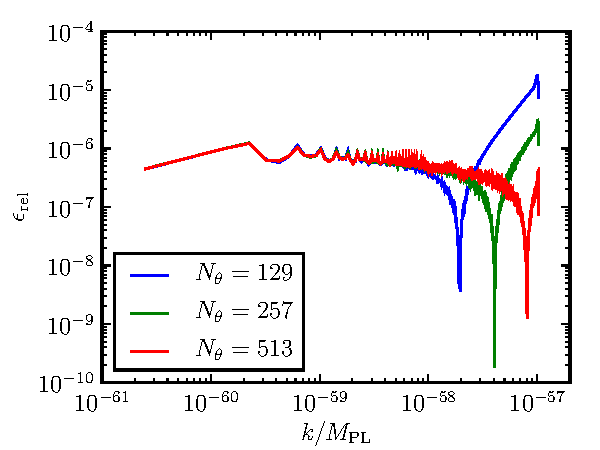
\includegraphics[width=0.43\textwidth]{numerical/graphs/err_nthetas-small.pdf}
 \label{fig:err-nthetas}
}\qquad
% 
\subfloat[Relative error for three different $k$ ranges][The relative error for the
three
different $k$ ranges $K_1$, $K_2$,
$K_3$ (starting from the left). The parameter $\Delta k$
is set equal to $1\e{-61}\Mpl, 3\e{-61}\Mpl, 1\e{-60}\Mpl$ respectively.]{
 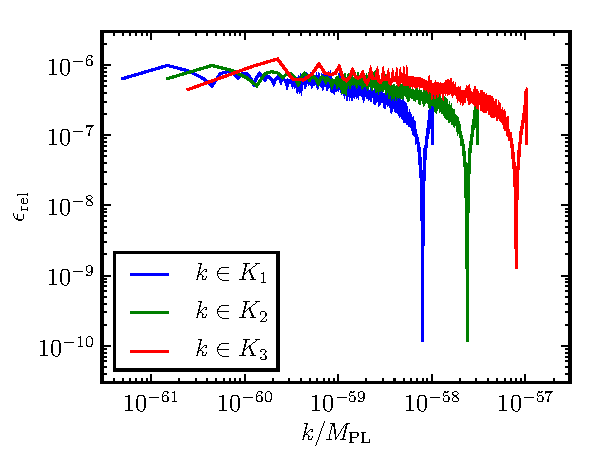
\includegraphics[width=0.43\textwidth]{numerical/graphs/err-kranges-small.pdf}
 \label{fig:err-kranges}
}
% 
\caption[Two figures comparing relative errors]{Comparison of relative errors for
different $N_\theta$ and $k$ ranges.}
\label{fig:err-comparison}
\end{figure}

\begin{figure}[htbp]
 \centering
 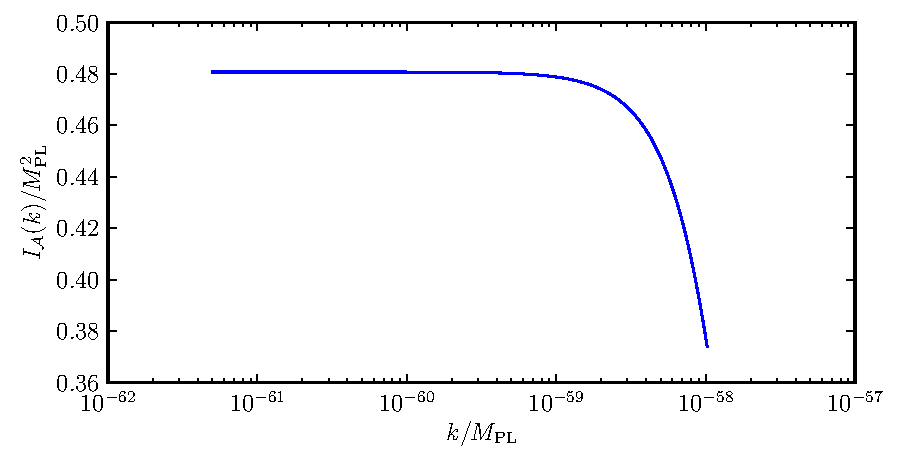
\includegraphics[width=0.8\textwidth]
    {./numerical/graphs/errors_analytic_aterm-half.pdf}
 % errors_analytic_aterm-half.pdf: 432x216 pixel, 72dpi, 15.24x7.62 cm
 \caption[The analytic solution of $I_\A$]{The analytic solution of $I_\A$ given in
\eq{eq:err-analytic-num} for
$k\in K_1$. The value of $\alpha$ is set as $2.7\e{57}$.}
 \label{fig:inta-num}
\end{figure}

The central calculation in the code is of the
convolution of the perturbations for the source term,
\eq{eq:KG2-source-ntime}. The first of the $\theta$ dependent terms in
\eq{eq:AtoD-num}, $\A$,
can be convolved analytically for certain smooth choices of $\dvp1(k)$. 
Taking $\dvp1(k)$ to be similar in form to the initial conditions
(\ref{eq:foics}) gives $\dvp1(k)\propto 1/\sqrt{k}$ with proportionality constant
$\alpha$.
If $I_\A$ denotes the convolution of the $\A$ term:
% 
\begin{equation}
 I_\A (k) = \int \d q^3 \dvp1(\qvi) \dvp1(\kvi-\qvi) 
          = 2\pi \int_{\kmin}^{\kmax} \d q\, q^2 \dvp1(\qvi) \A(\kvi, \qvi)\,,
\end{equation}
% 
then substituting $\dvp1(k) = \alpha/\sqrt{k}$ implies that
% 
\begin{equation}
 I_\A(k) = 2\pi\alpha^2 \int_{\kmin}^{\kmax} \d q\, q^{\frac{3}{2}}
\int_{0}^{\pi} \d\theta\, (k^2 + q^2 -2k q \cos{\theta})^{-1/4} \sin{\theta}\,. 
\end{equation}
% 
This has the analytic solution
% 
\begin{align}
\label{eq:err-analytic-num}
 I_\A(k) = -\frac{\pi\alpha^2}{18 k}\Bigg\{ 
	&3 k^3 \Bigg[ \log\Biggl(\frac{\sqrt{\kmax-k} + \sqrt{\kmax}}{\sqrt{k}}
			    \Biggr)
	 + \log\Biggl( \frac{\sqrt{k+\kmax} +\sqrt{\kmax}}{\sqrt{\kmin+k} +
		      \sqrt{\kmin}}\Biggr) \nonumber \\
	&+\frac{\pi}{2} - \arctan\left( \frac{\sqrt{\kmin}}{\sqrt{k-\kmin}}\right)
	\Bigg] \nonumber\\
% 
        &-\sqrt{\kmax}\Bigg[ \left(3k^2 + 8\kmax^2 \right)\left(\sqrt{k+\kmax} -
	  \sqrt{\kmax-k}\right) \nonumber \\
	&\qquad + 14k\kmax\left(\sqrt{k+\kmax}+\sqrt{\kmax-k}\right)\Bigg]\nonumber\\
% 
	&+\sqrt{\kmin}\Bigg[ \left(3k^2 + 8\kmin^2 \right)\left(\sqrt{k+\kmin} +
	  \sqrt{k-\kmin}\right) \nonumber \\
	&\qquad +14k\kmin \left(\sqrt{k+\kmin} -
         \sqrt{k-\kmin} \right) \Bigg] \Bigg\} \,.
\end{align}
% 
% 
% 
The $k$ dependence of $I_\A$ can be seen in Figure~\ref{fig:inta-num}. 
We have tested our code against this analytic solution for various
combinations of $k$ ranges and $N_\theta$. The relative error
%
\begin{equation}
 \epsilon_\mathrm{rel} = \frac{|\mathrm{analytic}- \mathrm{calculated}
|}{|\mathrm{analytic}|}
\end{equation}
%
is small for all the tested cases, but certain combinations of
parameters turn out to be more accurate than others. The relative error of
all the following results is not affected by the choice of $\alpha$ so
we will keep its numerical value fixed throughout as $2.7\e{57}$.

\begin{figure}[htbp]
 \centering
 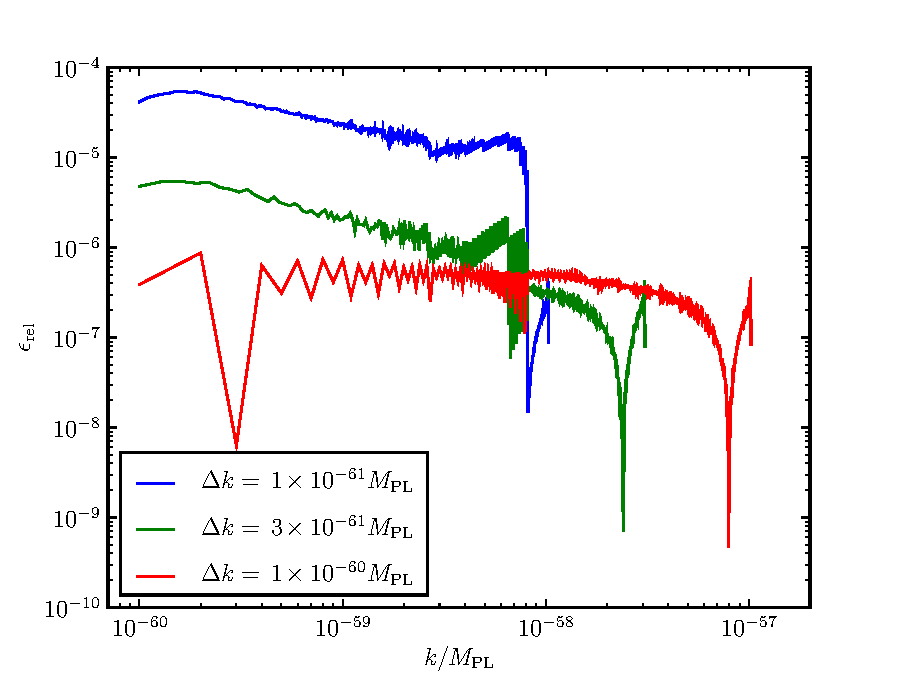
\includegraphics[width=0.8\textwidth]{numerical/graphs/err_deltaks-large}
 \caption[Relative error in the integral $I_\A$]{The relative error in the
integral $I_\A$ for different values of $\Delta k$.
The other parameters are fixed: $\kmin=1\times10^{-60}\Mpl, N_k = 1025$ and
$N_\theta=513$. 
The value of $\Delta k$ is less than $\kmin$ for the upper 
blue line ($\Delta k=1\e{-61}\Mpl$) and the middle green line ($\Delta
k=3\e{-61}\Mpl$). These have relative errors at least an order of magnitude larger
than the lower red line for which $\Delta k=\kmin=1\e{-60}\Mpl$.}
 \label{fig:err-deltaks}
\end{figure}


We first tested the effect of changing $N_\theta$, the number of
samples of the $\theta$ range $[0,\pi]$.  Figure~\ref{fig:err-nthetas}
plots these results for the $k$ range $K_3$ with $\Delta k =
1\e{-60}\Mpl$. Only three values of $N_\theta$ are shown for clarity. It
can be seen that increasing $N_\theta$ decreases the relative error when the other
parameters are kept constant, as one
might expect.


As mentioned above the choice of $k$ range is especially important as
the convolution of the terms depends strongly on the minimum and
maximum values of this range. Indeed, this is clear from the analytic
solution in \eq{eq:err-analytic-num}. Figure~\ref{fig:err-kranges}
shows the difference in relative error for the three different $k$
ranges described above with 
% Mpc values 
$\Delta k= 3.8\e{-5}, 1.2\e{-4}$ and $3.8\e{-4}\Mpc^{-1}$
% Mpl values
($\Delta k= 1\e{-61}, 3\e{-61},1\e{-60}\Mpl$),
respectively. The accuracy is similar in all three cases.


Another important check is whether the resolution of the $k$ range is
fine enough. Varying $\Delta k$ can not be done in isolation if the
constraint \eqref{eq:nk-constraint-num} for $N_k$ is to
be satisfied. For this test the end of the $k$ range was changed with $\Delta k$
but the other parameters were kept fixed at $\kmin=1\e{-60}\Mpl=3.8\e{-4}\Mpc^{-1},
N_k = 1025$ and $N_\theta=513$. Figure~\ref{fig:err-deltaks} plots
these results again for three indicative values.  For $\Delta
k<\kmin$, there is a marked degradation in
the accuracy of the method for the upper two lines. This is understandable as many
interpolations of multiples of $\Delta k$ below $\kmin$ will be set to
zero. Once $\Delta k$ is greater than $\kmin$, the relative error is
insensitive to further increases in the value of $\Delta k$. (This is not shown in
the figure.)


\begin{figure}[htbp]
 \centering
 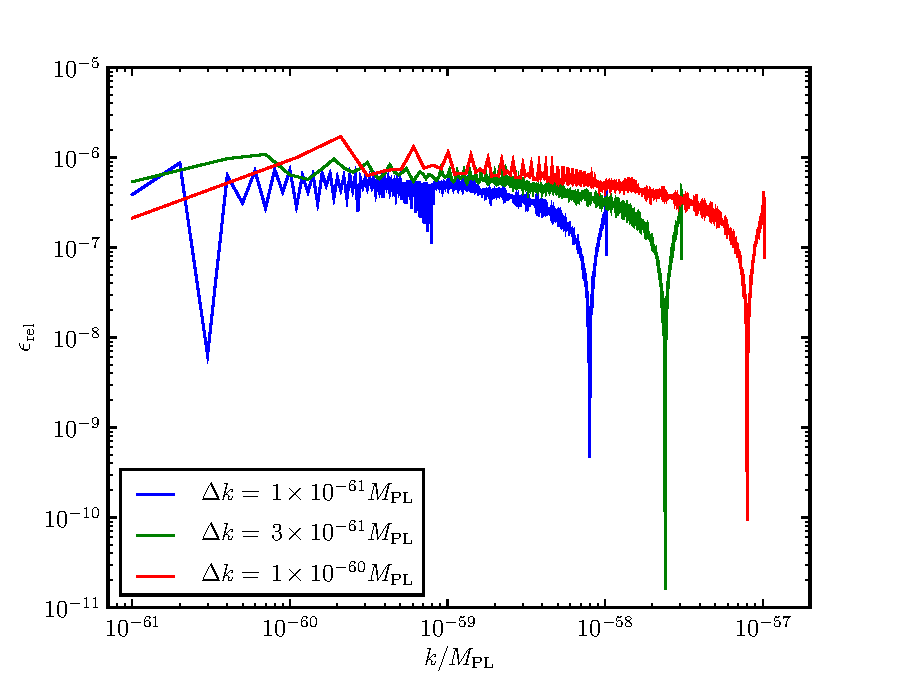
\includegraphics[width=0.8\textwidth]{numerical/graphs/err_deltak_kmin-large.pdf}
 % err-deltak-kmin.pdf: 432x324 pixel, 72dpi, 15.24x11.43 cm, bb=
 \caption[Relative error of $I_\A$ with fixed $\kmin$]{The 
relative error of the integral $I_\A$ for three different values of $\Delta k$. In
contrast to Figure~\ref{fig:err-deltaks}, $\kmin=1\e{-61}\Mpl=3.8\e{-5}\Mpc^{-1} \le
\Delta k$ for each case.}
 \label{fig:err-deltak-kmin}
\end{figure}
 
% 
% 
% Bterm
Analytic solutions can also be found for the $\B$, $\wt{\C}$ and $\wt{\D}$ terms.
The $\B$ term integral, $I_\B$, is given by
% 
\begin{align}
 \label{eq:bintegral-num}
I_\B &= 2\pi \int_{\kmin}^{\kmax} \d q\, q^2\dvp1(\qvi)\B(\kvi,\qvi) \nonumber\\
% 
     &= 2\pi\alpha^2 \int_{\kmin}^{\kmax} \d q\, q^{\frac{3}{2}}
\int_{0}^{\pi} \d\theta\, (k^2 + q^2 -2k q \cos{\theta})^{-1/4}
\cos{\theta}\sin{\theta}\,,
\end{align}
% 
and has the following analytic solution when $\dvp1(q) = \alpha/\sqrt{q}$:
% 
\begin{align}
\label{eq:intb-soln-num}
 I_\B = -\frac{\pi\alpha^2}{168 k^2}\Bigg\{ 
	&-63 k^4 \Bigg[ \log\Biggl(\frac{\sqrt{k}}{\sqrt{k+\kmin} + \sqrt{\kmin}}
			    \Biggr)
	 + \log\Biggl( \frac{\sqrt{k+\kmax} +\sqrt{\kmax}}{\sqrt{\kmax-k} +
		      \sqrt{\kmax}}\Biggr) \nonumber \\
	&-\frac{\pi}{2} + \arctan\left( \frac{\sqrt{\kmin}}{\sqrt{k-\kmin}}\right)
	\Bigg] \nonumber\\
% 
        &+\sqrt{\kmax}\Bigg[ \left(-65k^3 + 8k\kmax^2 \right)\left(\sqrt{k+\kmax} +
	  \sqrt{\kmax-k}\right) \nonumber \\
	&\qquad +\left(22k^2\kmax -16\kmax^3\right) \left(\sqrt{k+\kmax} -
         \sqrt{\kmax -k} \right) \Bigg] \nonumber \\
	&+\sqrt{\kmin}\Bigg[ \left(65k^3 - 8k\kmin^2 \right)\left(\sqrt{k+\kmin} -
	  \sqrt{k-\kmin}\right) \nonumber \\
	&\qquad +\left(-22k^2\kmin +16\kmin^3\right) \left(\sqrt{k+\kmin} +
         \sqrt{k-\kmin} \right) \Bigg] \Bigg\} \,.
\end{align}
% 
If, in addition to $\dvp1(q) = \alpha/\sqrt{q}$, we also take
% 
\begin{equation}
 \dN{\dvp1}(q) = -\frac{\alpha}{\sqrt{q}} -i\frac{\alpha\sqrt{q}}{\beta}\,
\end{equation}
% 
then the $\wt{\C}$ and $\wt{\D}$ terms can be integrated analytically.
The integral of the $\wt{\C}$ term is 
% 
\begin{align}
 \label{eq:cint-num}
I_{\wt{\C}} &= \int\d^3 q\, \dvp1(\qvi) \dN{\dvp1}(\kvi-\qvi) 
    = 2\pi \int \d q\, q^2 \dvp1(\qvi) \wt{\C}(\kvi, \qvi) \nonumber\\
% 
 &= -2\pi\alpha^2 \int_{\kmin}^{\kmax} \d q\, q^{\frac{3}{2}} \int_0^\pi 
     \left( \left(k^2 + q^2 -2kq \cos\theta\right)^{-\frac{1}{4}} \right.\nonumber \\
            &\qquad \qquad \left.+\frac{i}{\beta}\left(k^2 + q^2 -2kq
\cos\theta\right)^{\frac{1}{4}}
	\right) \sin\theta \d \theta\,,
\end{align}
% 
and the analytic solution is given by
% 
\begin{align}
\label{eq:cint-soln-num}
I_{\wt{\C}} = -I_\A -i\frac{\pi\alpha^2}{240 \beta k}\Bigg\{ 
	&15 k^4 \Bigg[ \log\Biggl(\frac{\sqrt{k+\kmin} + \sqrt{\kmin}}{\sqrt{k}}
			    \Biggr)
	 + \log\Biggl( \frac{\sqrt{\kmax-k} + \sqrt{\kmax}}{\sqrt{k+\kmax}
			+\sqrt{\kmax}}\Biggr) \nonumber \\
	&-\frac{\pi}{2} + \arctan\left( \frac{\sqrt{\kmin}}{\sqrt{k-\kmin}}\right)
	\Bigg] \nonumber\\
% 
        &+\sqrt{\kmax}\Bigg[ \left(15k^3 + 136k\kmax^2 \right)\left(\sqrt{k+\kmax} +
	  \sqrt{\kmax-k}\right) \nonumber \\
	&\qquad +\left(118k^2\kmax -48\kmax^3\right) \left(\sqrt{k+\kmax} -
         \sqrt{\kmax -k} \right) \Bigg] \nonumber \\
% 
	&-\sqrt{\kmin}\Bigg[ \left(15k^3 + 136k\kmin^2 \right)\left(\sqrt{k+\kmin} +
	  \sqrt{k-\kmin}\right) \nonumber \\
	&\qquad +\left(118k^2\kmin +48\kmin^3\right) \left(\sqrt{k+\kmin} -
         \sqrt{k-\kmin} \right) \Bigg] \Bigg\} \,.
\end{align}
 % 
The integral of the $\wt{\D}$ term is 
% 
\begin{align}
 \label{eq:dint-num}
I_{\wt{\D}} &= 2\pi \int \d q\, q^2 \dvp1(\qvi) \wt{\D}(\kvi, \qvi) \\
% 
 &= -2\pi\alpha^2 \int_{\kmin}^{\kmax} \d q\, q^{\frac{3}{2}} \int_0^\pi 
     \left( \left(k^2 + q^2 -2kq \cos\theta\right)^{-\frac{1}{4}} \right.\nonumber\\
% 
        &\qquad\qquad\left.+\frac{i}{\beta}\left(k^2 + q^2 -2kq
\cos\theta\right)^{\frac{1}{4}}
	\right) \cos\theta\sin\theta \d \theta\,,
\end{align}
% 
and the analytic solution is
% 
\begin{align}
\label{eq:dint-soln-num}
I_{\wt{\D}} = -I_\B &-i\frac{\pi\alpha^2}{900\beta k^2}\Bigg\{ \nonumber \\
	&135 k^5 \Bigg[ \log\Biggl(\frac{\sqrt{\kmax-k} + \sqrt{\kmax}}{\sqrt{k}}
			    \Biggr)
	 + \log\Biggl( \frac{\sqrt{k+\kmax} +\sqrt{\kmax}}{\sqrt{k+\kmin} +
			  \sqrt{\kmin}}\Biggr) \nonumber \\
	&\qquad -\frac{\pi}{2} + \arctan\left(
\frac{\sqrt{\kmin}}{\sqrt{k-\kmin}}\right)
	\Bigg] \nonumber\\
% 
        &-\sqrt{\kmax}\Bigg[ \left(-185k^4 + 168k^2\kmax^2-32\kmax^4
	    \right)\left(\sqrt{k+\kmax} - \sqrt{\kmax-k}\right) \nonumber \\
	&\qquad +\left(70k^3\kmax +16k\kmax^3\right) \left(\sqrt{k+\kmax} +
         \sqrt{\kmax -k} \right) \Bigg] \nonumber \\
% 
	&+\sqrt{\kmin}\Bigg[ \left(-185k^4 + 168k^2\kmin^2 -32\kmax^4
	    \right)\left(\sqrt{k+\kmin} - \sqrt{k-\kmin}\right) \nonumber \\
	&\qquad +\left(70k^3\kmin +16k\kmin^3\right) \left(\sqrt{k+\kmin} +
         \sqrt{k-\kmin} \right) \Bigg] \Bigg\} \,.
\end{align}
% 
The relative errors between the analytic and calculated values for $I_\B$,
$I_{\wt{\C}}$ and $I_{\wt{\D}}$ are shown in Figure~\ref{fig:rel-bcd-num} for the
three final $k$ ranges with $\beta=10^{-62}$. The errors
for the $I_{\wt{\C}}$ and $I_{\wt{\D}}$ terms are very small, being of the order of
$10^{-8}$ and $10^{-6}$, respectively. The relative error for the $I_\B$ term is
larger, especially for small $k$ values. However, the error is still below $0.08\%$
for each of the $K_1$, $K_2$ and $K_3$ ranges.


It should be noted that these tests only show the relative errors in the
computation of integrals of the four terms in \eq{eq:AtoD-num}. They
do not represent
errors for the full calculation. However, they do show that the accuracy is good
compared with the analytic result. 

\begin{figure}[htbp]
\centering%
\subfloat[The relative error for $I_\B$ for each $k$ range.]{
 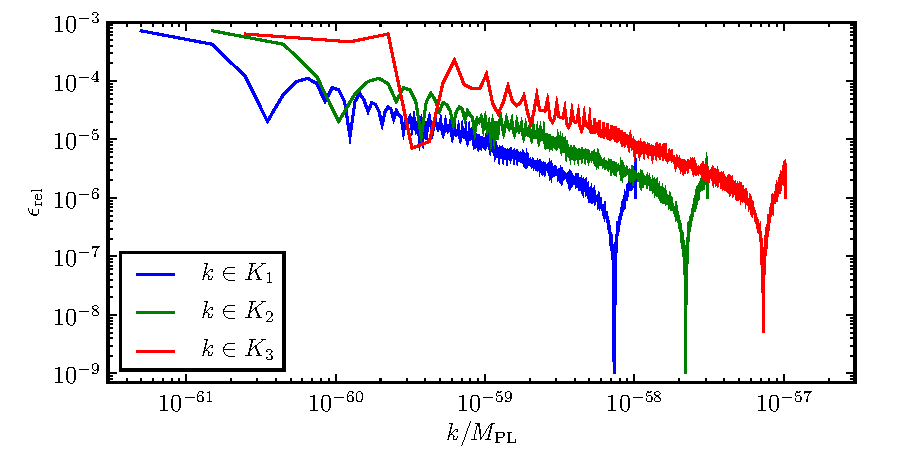
\includegraphics[width=0.8\textwidth]{numerical/graphs/errors_bterm-half}
}\\%
\subfloat[The relative error for $I_{\wt{\C}}$ for each $k$ range.]{
 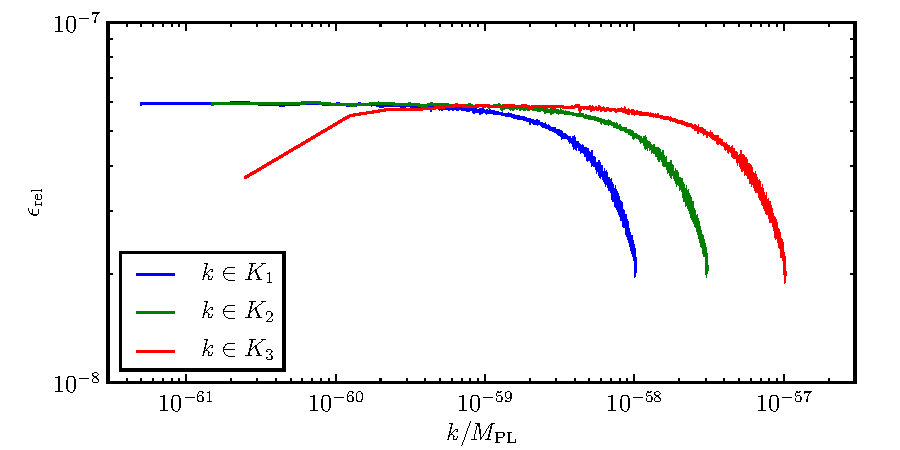
\includegraphics[width=0.8\textwidth]{numerical/graphs/errors_cterm-half}
}\\%
\subfloat[The relative error for $I_{\wt{\D}}$ for each $k$ range.]{
 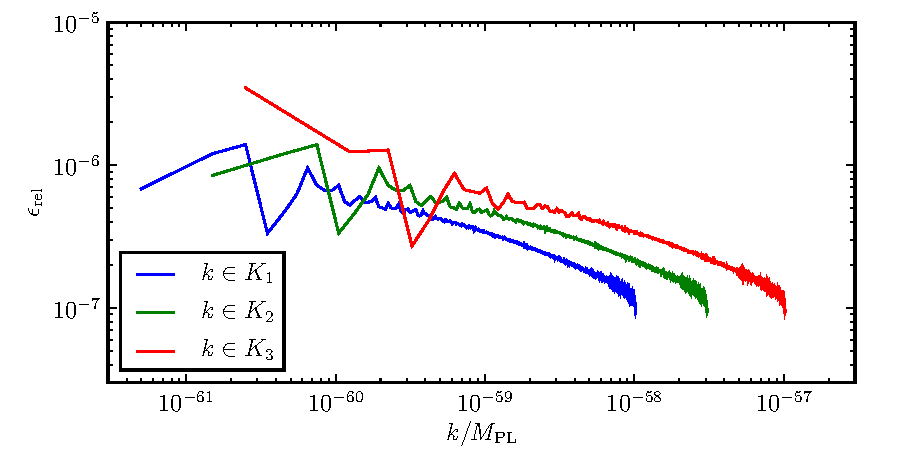
\includegraphics[width=0.8\textwidth]{numerical/graphs/errors_dterm-half}
}%
\caption[Relative errors for $I_\B$, $I_{\wt{\C}}$ and $I_{\wt{\D}}$]{The relative
errors for $I_\B$,
$I_{\wt{\C}}$ and $I_{\wt{\D}}$ for each of the $k$ ranges with $\beta=10^{-62}$.}
\label{fig:rel-bcd-num}
\end{figure}


% 
% 
% 

% % % % % % % % % % % % % % % % % % % % % % % % % % % % % % % % 
% =========================================================== %
% % % % % % % % % % % % % % % % % % % % % % % % % % % % % % % %
\section{Discussion}
\label{sec:disc-numerical}
% % % % % % % % % % % % % % % % % % % % % % % % % % % % % % % % 
% =========================================================== %
% % % % % % % % % % % % % % % % % % % % % % % % % % % % % % % %
This chapter has described the implementation of the numerical calculation of second
order cosmological perturbations.
The Klein-Gordon equations in Chapter~\ref{ch:perts} are the central focus of this
computation. In Section~\ref{sec:eqs-num} these equations were rewritten using $\N$
as the time variable, a choice more suitable for numerical work. The convolution
integrals in \eq{eq:KG2-fourier-sr-num} can be expressed in spherical polar
coordinates and split into four sub-terms $\A$--$\wt{\D}$ in \eqs{eq:AtoD-num} and
\eqref{eq:cdtilde-num}. Computing the source term
\eq{eq:KG2-source-ntime}, which is written using $\A$--$\wt{\D}$, is the most complex
and
time consuming part of the calculation.

To demonstrate the numerical code, four different potentials have been chosen and
these were described in Section~\ref{sec:pots-num}. One parameter for each
potential was determined by comparing the calculated $\Pr$ with the WMAP5 value.

In Section~\ref{sec:initconds-num} the initial conditions for the computed
quantities were explained. Each $k$ mode is initialised well inside the horizon
using the Bunch-Davies vacuum conditions from Section~\ref{sec:perts-intro}. The
second order perturbations are initially set to zero. This choice
concentrates focus
on the generation of second order effects during the observable period of
inflation.


The technical implementation of the code was discussed in
Section~\ref{sec:impl-num}. There are four stages in the procedure. First, the
background fields are evolved over a specified time period. The end time of
inflation is then determined by the condition $\varepsilon_H=1$ and the scale factor
calculated for this time. With this
information the initialisation of the first order modes can be performed. In the
second stage, the first order perturbation equations are solved. These results are
used in the third stage to calculate the source term \eq{eq:KG2-source-ntime} at each
time for each $k$. Finally, the second order perturbation equations are solved using
the source term results.

To test the source term calculation the numerical results were compared to 
analytic solutions in Section~\ref{sec:tests-num}. Numerical parameters such as
$N_\theta$ and $N_k$ were set by minimising the relative error between the two
approaches.

In Chapter~\ref{ch:perts} the evolution equations for second order perturbations
were introduced. In this chapter the practical implementation of a numerical
calculation of these perturbations was discussed. In Chapter~\ref{ch:results} the
results of this numerical calculation will be examined and the next steps towards an
improved procedure will be described.